\documentclass{beamer}

\usepackage{amsmath}
\usepackage{amsthm}
\usepackage[justification=raggedright,singlelinecheck=false]{caption}
\usepackage{graphicx}
\usepackage{hyperref}
\usepackage{natbib}
\usepackage{subcaption}

\usetheme{AnnArbor}
\graphicspath{{figures/}}
\hypersetup{colorlinks=true, citecolor=orange}
\setbeamertemplate{caption}[numbered]

\DeclareMathOperator*{\argmin}{arg\,min}
\newcommand{\E}{\mathbb{E}}
\newcommand{\Prob}{\mathbb{P}}
\newcommand{\R}{\mathbb{R}}

\title[Conformalized Quantile Regression]{
    Conformalized Quantile Regression
}
\author{Victor Verma}
\institute[]{
    Department of Statistics, University of Michigan
}
\date[10/17/25]{10/17/25}

\begin{document}

\begin{frame}
    \titlepage
\end{frame}

\begin{frame}{Today's Paper}
    Today's paper: ``Conformalized Quantile Regression''  \citep[][]{romano2019conf}.

    \medskip

    It introduces Conformalized Quantile Regression (CQR), a technique for producing prediction intervals. The main selling points of CQR:
    \begin{itemize}
        \item Unlike standard conformal prediction, CQR is adaptive to heteroskedasticity - the interval length can vary with the covariates.
        \item Just like standard conformal prediction, CQR has a marginal coverage guarantee.
        \item CQR tends to produce shorter intervals than alternative methods.
    \end{itemize}
\end{frame}

\begin{frame}{The Prediction Problem}
    We are given the below:
    \begin{description}
        \item[Training Set] $\{(X_i, Y_i)\}_{i = 1}^n \subset \R^p \times \R$, where
        \begin{itemize}
            \item $(X_1, Y_1), \ldots, (X_n, Y_n) \sim P_{X Y}$.
            \item $(X_1, Y_1), \ldots, (X_n, Y_n)$ are exchangeable.
        \end{itemize}
        \item[Miscoverage Rate] $\alpha \in (0, 1)$; $\alpha$ is close to zero.
    \end{description}

    The goal is to use the training data to construct an interval-valued function $C$ such that we have the following for a test point $(X_{n + 1}, Y_{n + 1})$:
    \begin{block}{Marginal Coverage Guarantee}
        $\Prob(Y_{n + 1} \in C(X_{n + 1})) \ge 1 - \alpha$.
    \end{block}
\end{frame}

\begin{frame}{Split Conformal Prediction: A Review}
    Split conformal prediction provides a means of constructing a $C$ for which the guarantee holds. First, the training set is split in two:
    \begin{description}
        \item[Proper Training Set] $\{(X_i, Y_i): i \in \mathcal{I}_1\}$
        \item[Calibration Set] $\{(X_i, Y_i): i \in \mathcal{I}_2\}$
    \end{description}

    These steps are then carried out:
    \begin{enumerate}
        \item Fit a regression model $\widehat{\mu}(x)$ to the proper training set.
        \item Compute residuals $R_i = |Y_i - \widehat{\mu}(X_i)|$, $i \in \mathcal{I}_2$, using the calibration set.
        \item Compute $Q_{1 - \alpha}(R, \mathcal{I}_2)$, the $(1 - \alpha)(1 + 1 / |\mathcal{I}_2|)$ quantile of the $R_i$'s.
        \item Compute $C(X_{n + 1})$ as
        \[
        [\widehat{\mu}(X_{n + 1}) - Q_{1 - \alpha}(R, \mathcal{I}_2), \widehat{\mu}(X_{n + 1}) + Q_{1 - \alpha}(R, \mathcal{I}_2)].
        \]
    \end{enumerate}
    \emph{A problem: the interval length is constant with respect to the covariates!}
\end{frame}

\begin{frame}[allowframebreaks]{Locally Adaptive Split Conformal Prediction}
    The constant length problem (a lack of adaptivity to heteroskedasticity) can be addressed using locally adaptive split conformal prediction. Data splitting is done as before, then these steps are carried out:
    \begin{enumerate}
        \item Fit a regression model $\widehat{\mu}(x)$ to the proper training set.
        \item Compute residuals $R_i = |Y_i - \widehat{\mu}(X_i)|$, $i \in \mathcal{I}_1$, using the \emph{proper training} set.
        \item Fit another model $\widehat{\sigma}(x)$ to $\{(X_i, R_i): i \in \mathcal{I}_1\}$.
        \item Compute residuals $\widetilde{R}_i = |Y_i - \widehat{\mu}(X_i)| / \widehat{\sigma}(X_i)$, $i \in \mathcal{I}_2$, using the \emph{calibration} set.
        \item Compute $Q_{1 - \alpha}(\widetilde{R}, \mathcal{I}_2)$, the $(1 - \alpha)(1 + 1 / |\mathcal{I}_2|)$ quantile of the $\widetilde{R}_i$'s.
        \item Compute $C(X_{n + 1})$ as
        \[
        [\widehat{\mu}(X_{n + 1}) - \widehat{\sigma}(X_{n + 1})Q_{1 - \alpha}(\widetilde{R}, \mathcal{I}_2), \widehat{\mu}(X_{n + 1}) + \widehat{\sigma}(X_{n + 1})Q_{1 - \alpha}(\widetilde{R}, \mathcal{I}_2)].
        \]
    \end{enumerate}

    \framebreak

    The interval length is no longer constant. However, this method has disadvantages:
    \begin{itemize}
        \item When the data is homoskedastic, the intervals tend to be too long (because of extra uncertainty stemming from the estimation of $\sigma(x)$?).
        \item The intervals tend not to be that adaptive. My interpretation of the argument at the end of Section 5:

        \medskip

        If $\widehat{\mu}(x)$ is a good model, then $R_i$, $i \in \mathcal{I}_1$, is small. Since $\widehat{\sigma}(x)$ is trained on $\{(X_i, R_i): i \in \mathcal{I}_1\}$, if $\widehat{\sigma}(x)$ is a good model, then $\widehat{\sigma}(X_i)$, $i \in \mathcal{I}_1$, is small. But if $\widehat{\sigma}(x)$ is generally small, then the interval length doesn't vary much with $X_{n + 1}$.
    \end{itemize}
\end{frame}

\begin{frame}[allowframebreaks]{Quantile Regression}
    The previous two methods construct $C(X_{n + 1})$ as a center $\widehat{\mu}(X_{n + 1})$ plus or minus a radius (e.g., $\widehat{\sigma}(X_{n + 1})Q_{1 - \alpha}(\widetilde{R}, \mathcal{I}_2)$). But the lower and upper endpoints could instead be constructed directly.

    \medskip

    Letting $q_{\alpha}(x)$ be the $\alpha$th quantile of $Y \mid X = x$ and $C(x) = [q_{\alpha / 2}(x), q_{1 - \alpha / 2}(x)]$, then we have the \emph{conditional} coverage guarantee
    \[
    \Prob(Y \in C(X) \mid X = x) \ge 1 - \alpha,
    \]
    and the length of $C(x)$ depends on $x$.

    \medskip

    Since we don't know $q_{\alpha}(x)$, we have to compute an estimate $\widehat{q}_{\alpha}(x)$ of it using quantile regression.

    \framebreak

    Recall that in quantile regression, $\widehat{q}_{\alpha}(x)$ is typically computed by solving the optimization problem
    \[
    \widehat{q}_{\alpha}(x) = f(x; \widehat{\theta}), \quad \widehat{\theta} = \argmin_{\theta} \frac{1}{n}\sum_{i = 1}^n \rho_{\alpha}(Y_i, f(x; \widehat{\theta})),
    \]
    where $\rho_{\alpha} : \R \to \R$ is defined by
    \[
    \rho_{\alpha}(t)
    =
    \begin{cases}
        \alpha t & \text{if} \ t \ge 0 \\
        (\alpha - 1)t & \text{if} \ t < 0.
    \end{cases}
    \]

    \framebreak

    Having computed $\widehat{q}_{\alpha / 2}(x)$ and $\widehat{q}_{1 - \alpha / 2}(x)$, we can construct
    \[
    \widehat{C}(X_{n + 1}) = [\widehat{q}_{\alpha / 2}(X_{n + 1}), \widehat{q}_{1 - \alpha / 2}(X_{n + 1})].
    \]
    This interval is adaptive to heteroskedasticity, but neither conditional nor marginal coverage are guaranteed.

    \medskip

    However, marginal coverage can be guaranteed if the endpoints of $\widehat{C}(X_{n + 1})$ are adjusted.
\end{frame}

\begin{frame}[allowframebreaks]{Split Conformalized Quantile Regression}
    Split Conformalized Quantile Regression (CQR) adjusts the endpoints to obtain the marginal coverage guarantee.

    \medskip

    Data splitting is done as before, and then these steps are performed:
    \begin{enumerate}
        \item Fit quantile regression models $\widehat{q}_{\alpha / 2}(x)$ and $\widehat{q}_{1 - \alpha / 2}(x)$ to the proper training set.
        \item Compute conformity scores $E_i = \max\{\widehat{q}_{\alpha / 2}(X_i) - Y_i, Y_i - \widehat{q}_{1 - \alpha / 2}(X_i)\}$, $i \in \mathcal{I}_2$, using the calibration set.
        \item Compute $Q_{1 - \alpha}(E, \mathcal{I}_2)$, the $(1 - \alpha)(1 + 1 / |\mathcal{I}_2|)$ quantile of the $E_i$'s.
        \item Compute $C(X_{n + 1})$ as
        \[
        [\widehat{q}_{\alpha / 2}(X_{n + 1}) - Q_{1 - \alpha}(E, \mathcal{I}_2), \widehat{q}_{1 - \alpha / 2}(X_{n + 1}) + Q_{1 - \alpha}(E, \mathcal{I}_2)].
        \]
    \end{enumerate}

    \framebreak

    Some observations about $E_i = \max\{\widehat{q}_{\alpha / 2}(X_i) - Y_i, Y_i - \widehat{q}_{1 - \alpha / 2}(X_i)\}$:
    \begin{itemize}
        \item If $Y_i \notin [\widehat{q}_{\alpha / 2}(X_i), \widehat{q}_{1 - \alpha / 2}(X_i)]$, then $E_i > 0$.
        \begin{itemize}
            \item If $Y_i < \widehat{q}_{\alpha / 2}(X_{n + 1})$, then $E_i = \widehat{q}_{\alpha / 2}(X_i) - Y_i > 0$.
            \item If $Y_i > \widehat{q}_{1 - \alpha / 2}(X_i)$, then $E_i = Y_i - \widehat{q}_{1 - \alpha / 2}(X_i) > 0$.
        \end{itemize}
        \item If $Y_i \in [\widehat{q}_{\alpha / 2}(X_i), \widehat{q}_{1 - \alpha / 2}(X_i)]$, then $E_i \le 0$, as $\widehat{q}_{\alpha / 2}(X_i) - Y_i \le 0, \ Y_i - \widehat{q}_{1 - \alpha / 2}(X_i) \le 0$.
    \end{itemize}

    The adjustment of $Q_{1 - \alpha}(E, \mathcal{I}_2)$ addresses both over- and undercoverage:
    \begin{description}
        \item[Overcoverage] $Y_i \in [\widehat{q}_{\alpha / 2}(X_i), \widehat{q}_{1 - \alpha / 2}(X_i)]$ for more than $(1 - \alpha)$ $i \in \mathcal{I}_2$; $E_i \le 0$ for these $i$, so $Q_{1 - \alpha}(E, \mathcal{I}_2) \le 0$, and $C(X_{n + 1})$ is narrower.
        \item[Undercoverage] $Y_i \in [\widehat{q}_{\alpha / 2}(X_i), \widehat{q}_{1 - \alpha / 2}(X_i)]$ for less than $(1 - \alpha)$ $i \in \mathcal{I}_2$; $E_i \le 0$ for these $i$, so $Q_{1 - \alpha}(E, \mathcal{I}_2) > 0$, and $C(X_{n + 1})$ is wider.
    \end{description}

    \framebreak

    Split CQR has the marginal coverage guarantee:
    \begin{theorem}[Theorem 1 in \cite{romano2019conf}]
        If $(X_i, Y_i)$, $i = 1, \ldots, n + 1$ are exchangeable, then the prediction interval $C(X_{n + 1})$ constructed by the split CQR algorithm satisfies
        \[
        \Prob(Y_{n + 1} \in C(X_{n + 1})) \ge 1 - \alpha.
        \]
        Moreover, if the conformity scores $E_i$ are almost surely distinct, then the prediction interval is nearly perfectly calibrated:
        \[
        \Prob(Y_{n + 1} \in C(X_{n + 1})) \le 1 - \alpha + 1/(|\mathcal{I}_2| + 1).
        \]
    \end{theorem}
\end{frame}

\begin{frame}[allowframebreaks]{An Improved Variant of Split CQR}
    Split CQR ``allows coverage errors to be spread arbitrarily over the left and right tails.'' (?). A stronger coverage guarantee can be obtained by controlling the left and right tails independently. The steps are as follows:

    \begin{enumerate}
        \item Fit quantile regression models $\widehat{q}_{\alpha_{\text{lo}}}(x)$ and $\widehat{q}_{\alpha_{\text{hi}}}(x)$ to the proper training set.
        \item Compute conformity scores $E_{\text{lo}, i} = \widehat{q}_{\alpha_{\text{lo}}}(X_i) - Y_i$ and $E_{\text{hi}, i} = Y_i - \widehat{q}_{\alpha_{\text{hi}}}(X_i)$, $i \in \mathcal{I}_2$, using the calibration set.
        \item Compute $Q_{1 - \alpha_{\text{lo}}}(E_{\text{lo}}, \mathcal{I}_2)$ and $Q_{1 - \alpha_{\text{hi}}}(E_{\text{hi}}, \mathcal{I}_2)$, the $(1 - \alpha_{\text{lo}})$ quantile of the $E_{\text{lo}, i}$'s and the $(1 - \alpha_{\text{hi}})$ quantile of the $E_{\text{hi}, i}$'s.
        \item Compute $C(X_{n + 1})$ as
        \[
        [\widehat{q}_{\alpha_{\text{lo}}}(X_{n + 1}) - Q_{1 - \alpha_{\text{lo}}}(E_{\text{lo}}, \mathcal{I}_2), \widehat{q}_{\alpha_{\text{hi}}}(X_{n + 1}) + Q_{1 - \alpha_{\text{hi}}}(E_{\text{hi}}, \mathcal{I}_2)].
        \]
    \end{enumerate}

    \framebreak

    This variant has this marginal coverage guarantee:
    \begin{theorem}[Theorem 1]
        If $(X_i, Y_i)$, $i = 1, \ldots, n + 1$ are exchangeable, then the prediction interval $C(X_{n + 1})$ constructed by the variant of the split CQR algorithm satisfies
        \begin{align*}
            \Prob(Y_{n + 1} \ge \widehat{q}_{\alpha_{\text{lo}}}(X_{n + 1}) - Q_{1 - \alpha_{\text{lo}}}(E_{\text{lo}}, \mathcal{I}_2)) &\ge 1 - \alpha_{\text{lo}} \\
            \Prob(Y_{n + 1} \le \widehat{q}_{\alpha_{\text{hi}}}(X_{n + 1}) + Q_{1 - \alpha_{\text{hi}}}(E_{\text{hi}}, \mathcal{I}_2) &\ge 1 - \alpha_{\text{hi}}.
        \end{align*}
    \end{theorem}
    Note that if we set $\alpha = \alpha_{\text{lo}} + \alpha_{\text{hi}}$, then we get the original guarantee:
    \begin{align*}
        \Prob(Y_{n + 1} \notin C(X_{n + 1})) &= \Prob(Y_{n + 1} < \widehat{q}_{\alpha_{\text{lo}}}(X_{n + 1}) - Q_{1 - \alpha_{\text{lo}}}(E_{\text{lo}}, \mathcal{I}_2)) \\
        &\quad + \Prob(Y_{n + 1} > \widehat{q}_{\alpha_{\text{hi}}}(X_{n + 1}) + Q_{1 - \alpha_{\text{hi}}}(E_{\text{hi}}, \mathcal{I}_2) \\
        &\le \alpha_{\text{lo}} + \alpha_{\text{hi}} \\
        &\le \alpha.
    \end{align*}
\end{frame}

\begin{frame}[allowframebreaks]{Experiment: Heteroscedastic Data with Outliers}
    $n = 7000$ $(X, Y)$ pairs were generated using the following procedure:
    \begin{enumerate}
        \item Draw a random sample $\{X_1, \ldots, X_n\}$ from the $\text{Unif}[1, 5]$ distribution.
        \item For $i = 1, \ldots, n$, generate $Y_i$ using
        \[
        Y_i = \text{Pois}(\sin^2(X_i) + 0.1) + 0.03 X_i\epsilon_{1, i} + 25\mathbb{I}\{U_i < 0.01\}\epsilon_{2, i},
        \]
        where $\epsilon_{1, i}, \epsilon_{2, i} \overset{\text{iid}}{\sim} \text{Norm}(0, 1)$ and $U_i \sim \text{Unif}[0, 1]$.
    \end{enumerate}

    The first $2000$ pairs were used for training and the last $5000$ for testing.

    More details:
    \begin{itemize}
        \item $\alpha = 0.1$.
        \item $\widehat{\mu}(x), \widehat{\sigma}(x)$: random forests.
        \item $\widehat{q}_{\alpha / 2}(x), \widehat{q}_{1 - \alpha / 2}(x)$: quantile random forests.
    \end{itemize}

    \framebreak

    \begin{figure}
        \centering
        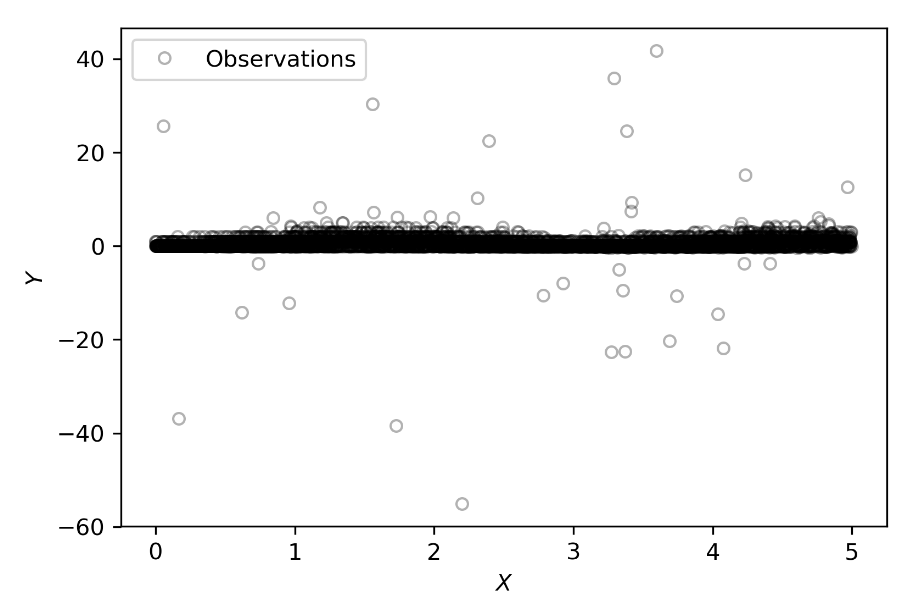
\includegraphics[scale=0.58]{romano_et_al/fig_a1.png}
        \caption{Figure 1 in the supplement for \cite{romano2019conf}.}
        \label{fig:romano_et_al_fig_a1}
    \end{figure}

    \framebreak

    \begin{figure}
        \centering
        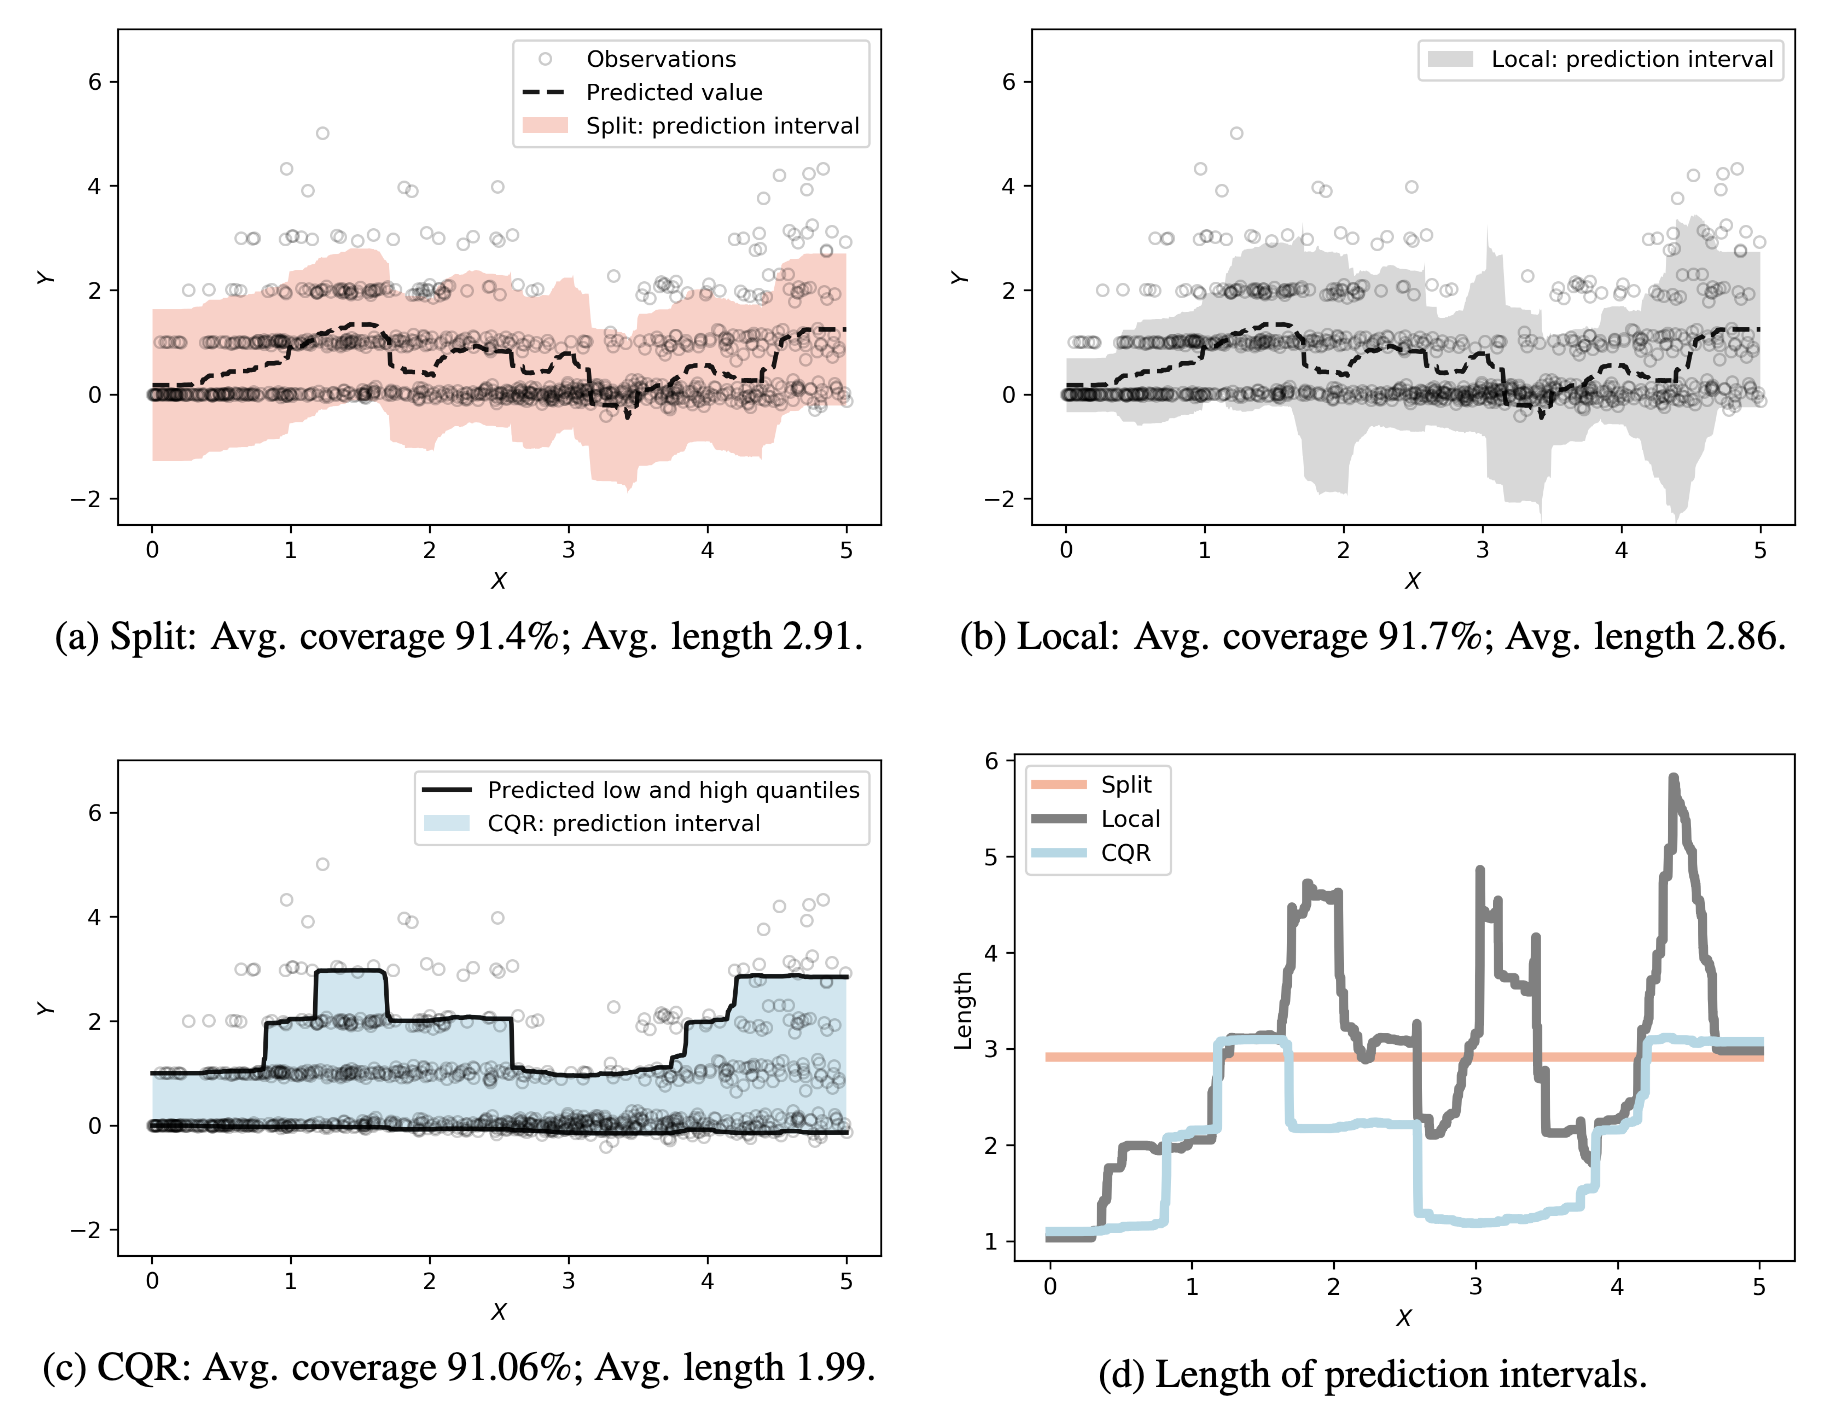
\includegraphics[scale=0.25]{romano_et_al/fig_1.png}
        \caption{Figure 1 in \cite{romano2019conf}.}
        \label{fig:romano_et_al_fig_1}
    \end{figure}
\end{frame}

\begin{frame}[allowframebreaks]{Experiment: Heavy-Tailed Cauchy Distribution}
    $n = 7000$ $(X, Y)$ pairs were generated using the following procedure:
    \begin{enumerate}
        \item Draw a random sample $\{X_1, \ldots, X_n\}$ from the $\text{Unif}[0, 10]$ distribution.
        \item For $i = 1, \ldots, n$, generate $Y_i$ using
        \[
        Y_i \sim \text{Cauchy}(0, 6 \sin^2(X_i)),
        \]
        where $0$ is the location parameter and $6 \sin^2(X_i)$ is the scale parameter.
    \end{enumerate}
    The first $2000$ pairs were used for training and the last $5000$ for testing.

    More details:
    \begin{itemize}
        \item $\alpha = 0.1$.
        \item $\widehat{\mu}(x), \widehat{\sigma}(x)$: random forests.
        \item $\widehat{q}_{\alpha / 2}(x), \widehat{q}_{1 - \alpha / 2}(x)$: quantile random forests.
    \end{itemize}

    \framebreak

    \begin{figure}
        \centering
        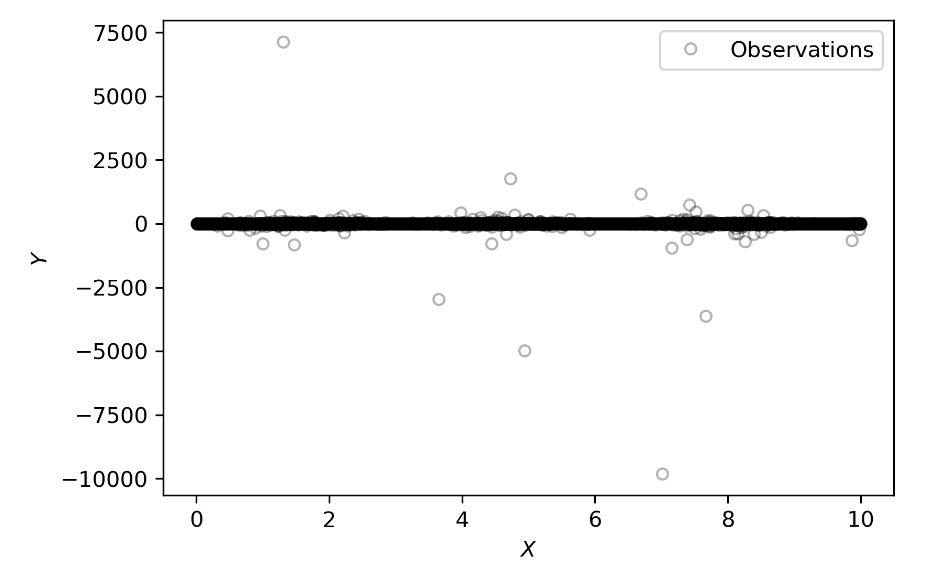
\includegraphics[scale=0.58]{romano_et_al/fig_a3.png}
        \caption{Figure 3 in the supplement for \cite{romano2019conf}.}
        \label{fig:romano_et_al_fig_a3}
    \end{figure}

    \framebreak

    \begin{figure}
        \centering
        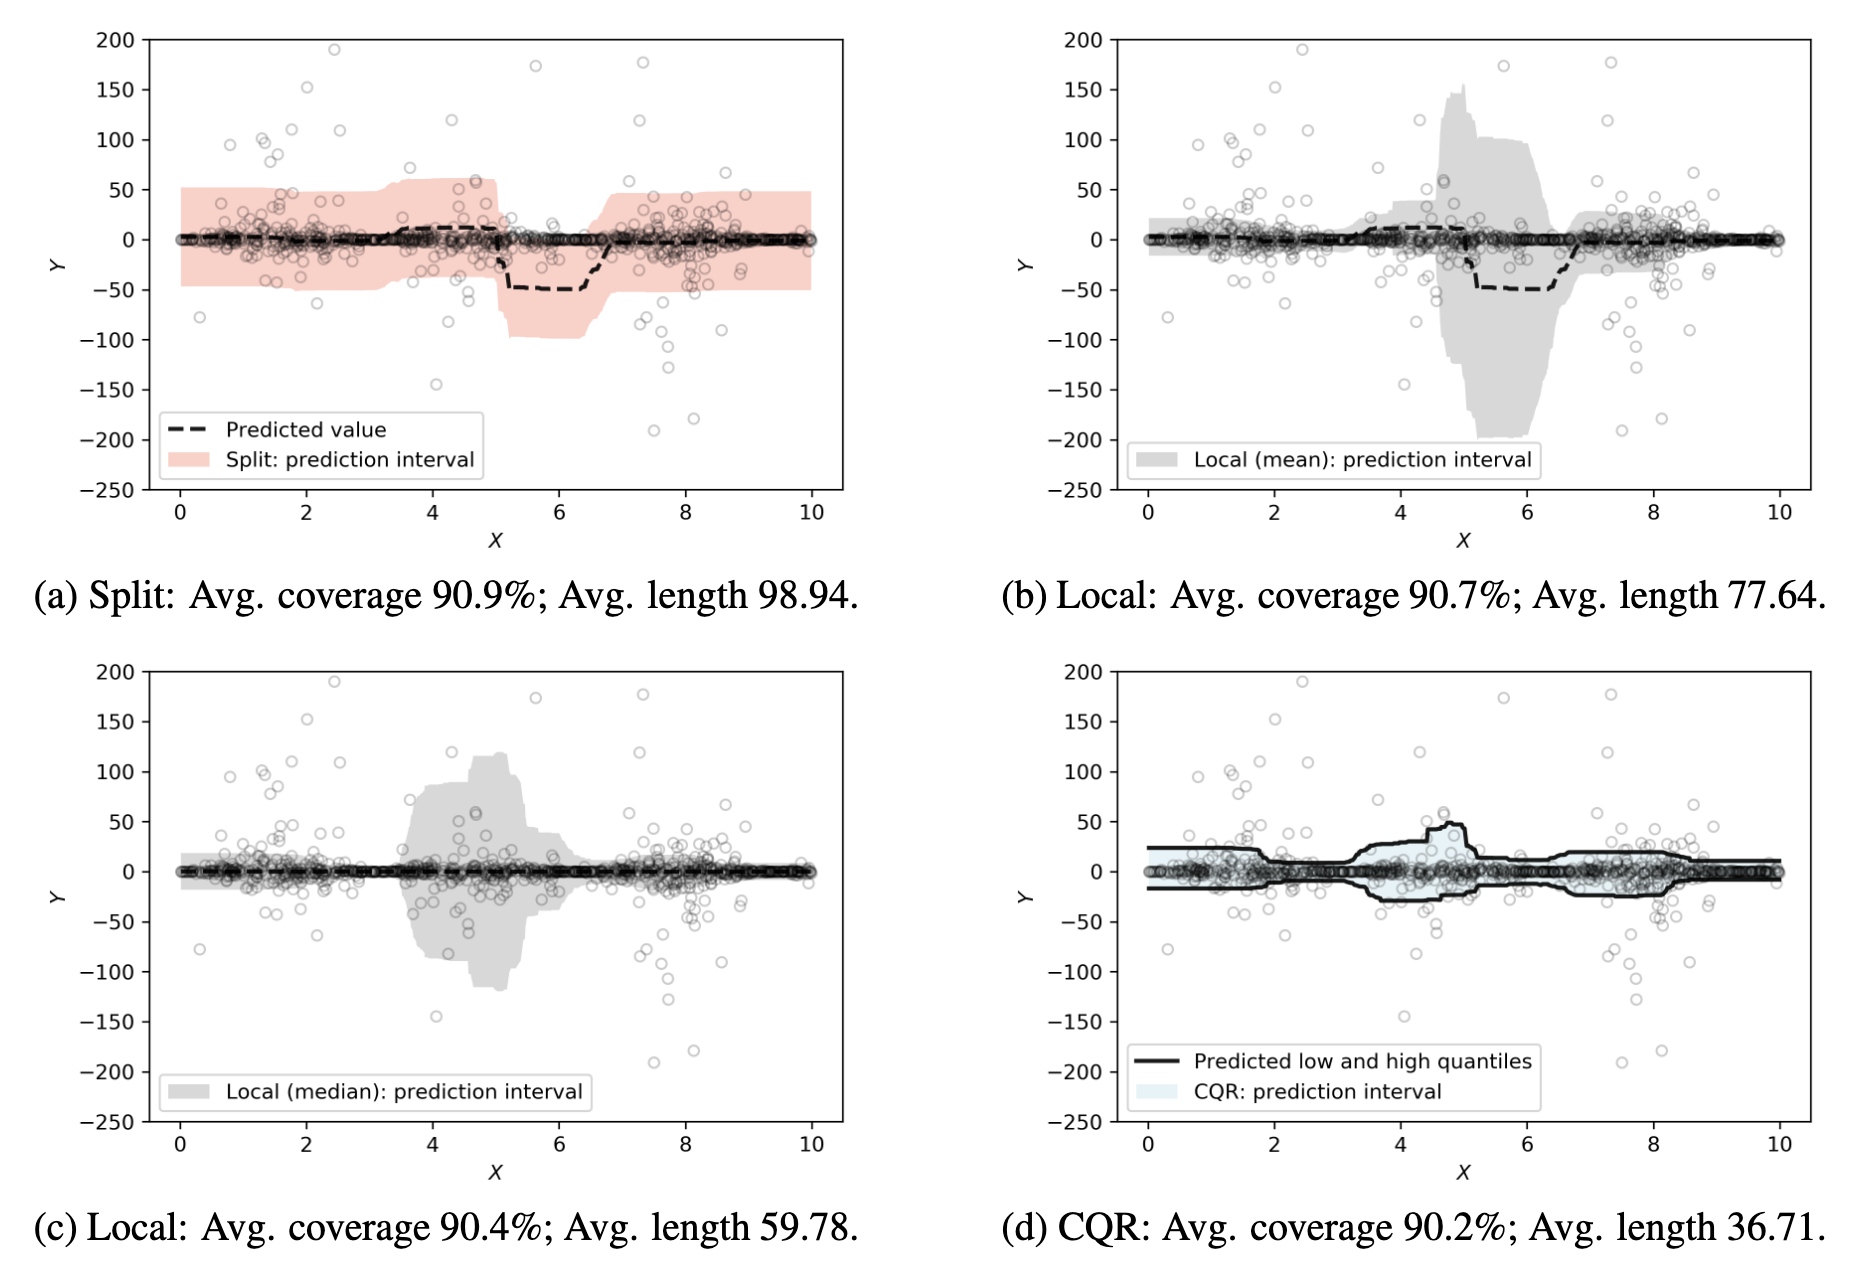
\includegraphics[scale=0.25]{romano_et_al/fig_a4.png}
        \caption{Figure 4 in the supplement for \cite{romano2019conf}.}
        \label{fig:romano_et_al_fig_a4}
    \end{figure}
\end{frame}

\begin{frame}[allowframebreaks]{Experiment: Real Datasets}
    An experiment was performed involving 11 benchmark real datasets.
    \begin{itemize}
        \item Each dataset was split into a proper training set ($40\%$), a calibration set ($40\%$), and a test set ($20\%$).
        \item Splitting was done 20 times, and performance metrics were averaged over the splits.
        \item $\alpha$ was fixed at $0.1$.
    \end{itemize}
    The following methods were used:
    \begin{itemize}
        \item Split conformal prediction based on ridge regression, random forests, and neural networks.
        \item Locally adaptive split conformal prediction based on ridge regression, random forests, and neural networks.
        \item Split CQR based on quantile random forests and quantile neural networks.
    \end{itemize}

    \framebreak

    \begin{figure}
        \centering
        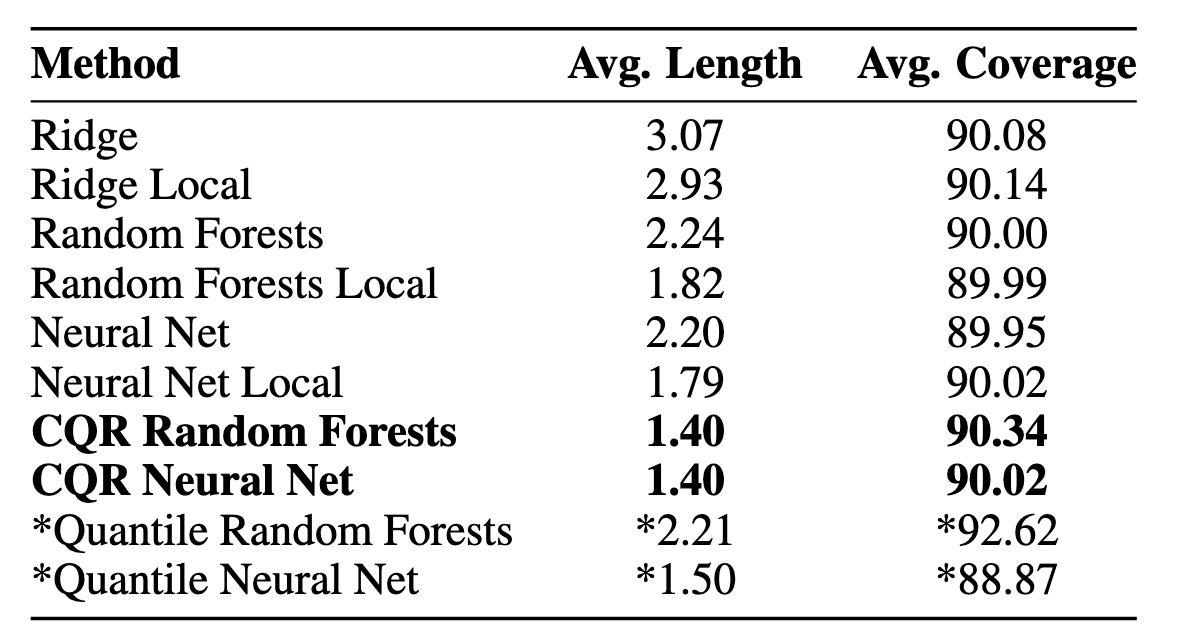
\includegraphics[scale=0.5]{romano_et_al/tab_1.png}
        \caption{Table 1 in \cite{romano2019conf}.}
        \label{fig:romano_et_al_tab_1}
    \end{figure}

    \framebreak

    \begin{figure}
        \centering
        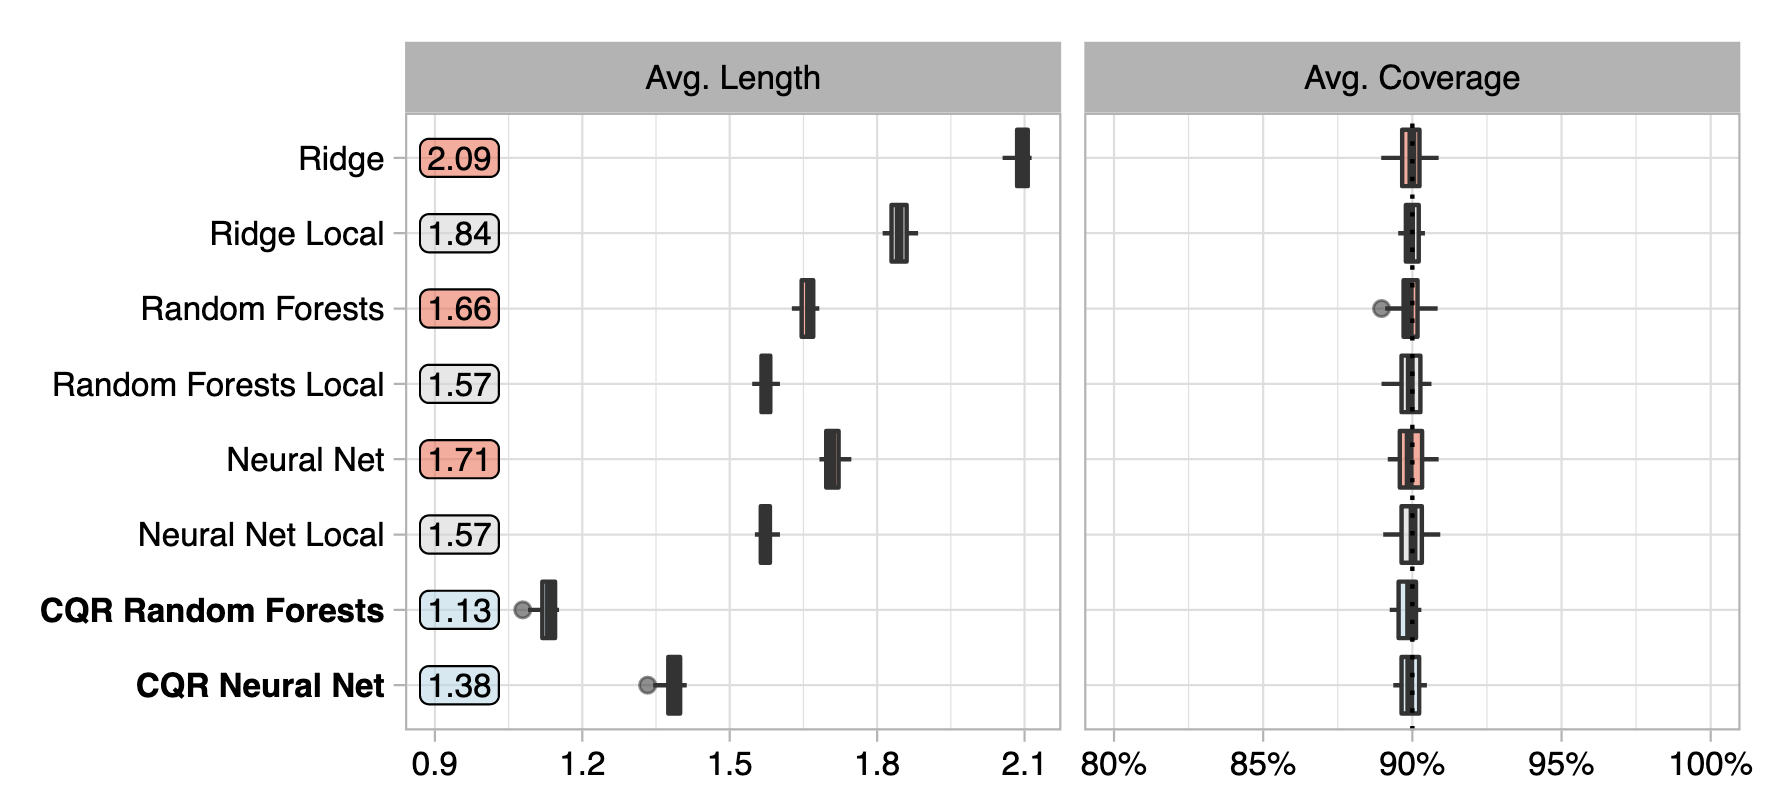
\includegraphics[scale=0.37]{romano_et_al/fig_2.png}
        \caption{Figure 2 in \cite{romano2019conf}.}
        \label{fig:romano_et_al_fig_2}
    \end{figure}
\end{frame}

\begin{frame}{More Variants of Split CQR: Split CQR-M}
    CQR-M, introduced in \cite{kivaranovic2020adap}, has these steps:
    \begin{enumerate}
        \item Fit quantile regression models $\widehat{q}_{1 / 2}(x)$, $\widehat{q}_{\alpha / 2}(x)$, and $\widehat{q}_{1 - \alpha / 2}(x)$ to the proper training set.
        \item Compute conformity scores using the calibration set:
        \[
        E_i = \max\left\{\frac{\widehat{q}_{\alpha / 2}(X_i) - Y_i}{\widehat{q}_{1 / 2}(X_i) - \widehat{q}_{\alpha / 2}(X_i)}, \frac{Y_i - \widehat{q}_{1 - \alpha / 2}(X_i)}{\widehat{q}_{1 - \alpha / 2}(X_i) - \widehat{q}_{1 / 2}(X_i)}\right\}, \ i \in \mathcal{I}_2.
        \]
        \item Compute $Q_{1 - \alpha}(E, \mathcal{I}_2)$, the $(1 - \alpha)(1 + 1 / |\mathcal{I}_2|)$ quantile of the $E_i$'s.
        \item Compute $C(X_{n + 1})$ as
        \begin{multline*}
            [\widehat{q}_{\alpha / 2}(X_{n + 1}) - Q_{1 - \alpha}(E, \mathcal{I}_2)
               [\widehat{q}_{1 / 2}(X_i) - \widehat{q}_{\alpha / 2}(X_i)], \\
            \widehat{q}_{1 - \alpha / 2}(X_{n + 1}) + Q_{1 - \alpha}(E, \mathcal{I}_2)
               [\widehat{q}_{1 - \alpha / 2}(X_i) - \widehat{q}_{1 / 2}(X_i)]].
        \end{multline*}
    \end{enumerate}
\end{frame}

\begin{frame}{More Variants of Split CQR: Split CQR-R}
    CQR-R, introduced in \cite{sesia2020comp}, has these steps:
    \begin{enumerate}
        \item Fit quantile regression models $\widehat{q}_{\alpha / 2}(x)$, and $\widehat{q}_{1 - \alpha / 2}(x)$ to the proper training set.
        \item Compute conformity scores using the calibration set:
        \[
        E_i = \max\left\{\frac{\widehat{q}_{\alpha / 2}(X_i) - Y_i}{\widehat{q}_{1 - \alpha / 2}(X_i) - \widehat{q}_{\alpha / 2}(X_i)}, \frac{Y_i - \widehat{q}_{1 - \alpha / 2}(X_i)}{\widehat{q}_{1 - \alpha / 2}(X_i) - \widehat{q}_{\alpha / 2}(X_i)}\right\}, \ i \in \mathcal{I}_2.
        \]
        \item Compute $Q_{1 - \alpha}(E, \mathcal{I}_2)$, the $(1 - \alpha)(1 + 1 / |\mathcal{I}_2|)$ quantile of the $E_i$'s.
        \item Compute $C(X_{n + 1})$ as
        \begin{multline*}
            [\widehat{q}_{\alpha / 2}(X_{n + 1}) - Q_{1 - \alpha}(E, \mathcal{I}_2)
               [\widehat{q}_{1 - \alpha / 2}(X_i) - \widehat{q}_{\alpha / 2}(X_i)], \\
            \widehat{q}_{1 - \alpha / 2}(X_{n + 1}) + Q_{1 - \alpha}(E, \mathcal{I}_2)
               [\widehat{q}_{1 - \alpha / 2}(X_i) - \widehat{q}_{\alpha / 2}(X_i)]].
        \end{multline*}
    \end{enumerate}
\end{frame}

\begin{frame}[allowframebreaks]{Theoretical Results for Split CQR, CQR-M, CQR-R}
    Split CQR, CQR-M, and CQR-R have the marginal coverage guarantee.

    \medskip

    It is shown in \cite{sesia2020comp} that for split CQR, CQR-M, and CQR-R, as the amount of data increases, $C(X_{n + 1}) \to [q_{\alpha / 2}(x), q_{1 - \alpha / 2}(x)]$.

    \smallskip

    To formalize this, the assumptions below are needed:
    \begin{itemize}
        % [iid]
        \item The points $\{(X_i, Y_i)\}_{i = 1}^{n + 1}$ are drawn iid from some distribution $P_{X Y}$. 
        % [Regularity]
        \item The probability density of the conformity scores is bounded away from zero in an open neighborhood of zero.
        % [Consistency]
        \item Let $n_1 = |\mathcal{I}_1|$ and $X$ be a new observation independent of $I_1$. Then there exist sequences $\eta_{n_1}, \rho_{n_1} = o(1)$, $n_1 \to \infty$, such that large enough $n_1$,
        \begin{align*}
            \Prob\left(
                \E\left[\bigl(\hat q_{\alpha/2}(X) - q_{\alpha/2}(X)\bigr)^2
                \,\middle|\, \hat q_{\alpha/2}, \hat q_{1-\alpha/2}\right]
                \le \eta_{n_1}
            \right) &\ge 1 - \rho_{n_1} \\
            \Prob\left(
                \E\left[\bigl(\hat q_{1-\alpha/2}(X) - q_{1-\alpha/2}(X)\bigr)^2
                \,\middle|\, \hat q_{\alpha/2}, \hat q_{1-\alpha/2}\right]
                \le \eta_{n_1}
            \right) &\ge 1 - \rho_{n_1}.
        \end{align*}
    \end{itemize}

    \framebreak

    It can be shown that $\hat q_{\alpha/2}(X) \xrightarrow{L^2} q_{\alpha/2}(X)$ and $\hat q_{1-\alpha/2}(X) \xrightarrow{L^2} q_{1-\alpha/2}(X)$ imply the third assumption.

    \medskip

    For split CQR, CQR-M, and CQR-R, the following result holds:
    \begin{theorem}[Theorem 1 in \cite{sesia2020comp}]
        Under the three assumptions, $C(X_{n + 1})$ satisfies
        \[
        \lambda(C(X_{n + 1}) \triangle [q_{\alpha / 2}(x), q_{1 - \alpha / 2}(x)]) = o_P(1)
        \]
        as $|\mathcal{I}_1|, |\mathcal{I}_2| \to \infty$, where $\lambda$ is Lebesgue measure.
    \end{theorem}

    \framebreak

    We also have this result for split CQR, CQR-M, and CQR-R:
    \begin{corollary}[Corollary 1 in \cite{sesia2020comp}]
        Under the three assumptions and the assumption that $Y$ has a continuous density with respect to $\lambda$,
        \[
        \sup_{x \in \Lambda_n}
        \bigg| \Prob\!\big( Y \in \widehat{C}_n(x)\,\big|\, X = x \big) - (1-\alpha) \bigg|
        \;=\; o_P(1),
        \]
        where $\{\widehat{C}_n\}$ is a sequence of (random) prediction bands and $\Lambda_n \subseteq \R^d$ is a sequence of (random) sets with $\Prob\!\big(X \in \Lambda_n\big) = 1 - o_P(1)$.
    \end{corollary}
\end{frame}

\begin{frame}[allowframebreaks]{Experiment: Real Datasets}
    In \cite{sesia2020comp}, split CQR, CQR-M, and CQR-R were compared using the same 11 real datasets that were used in \cite{romano2019conf}.
    \begin{itemize}
        \item The proportion of training data $\gamma$ put in $\mathcal{I}_1$ was varied:
        \[
        \gamma \in \{0.1, 0.25, 0.5, 0.6, 0.7, 0.8, 0.9, 0.95, 0.98\}.
        \]
        $20\%$ of the data was always used for testing.
        \item Data splitting was repeated 10 times.
        \item For each split CQR variant, the $\gamma$ value leading to the shortest average interval length was computed.
        \item The impact of $\gamma$ on interval length and coverage was also assessed.
        \begin{itemize}
            \item Conclusion: use a $\gamma \in [0.7, 0.9]$.
        \end{itemize}
    \end{itemize}

    \framebreak

    \begin{figure}
        \captionsetup[subfigure]{justification=centering,singlelinecheck=true}
        \centering
        \begin{subfigure}{0.485\textwidth}
            \centering
            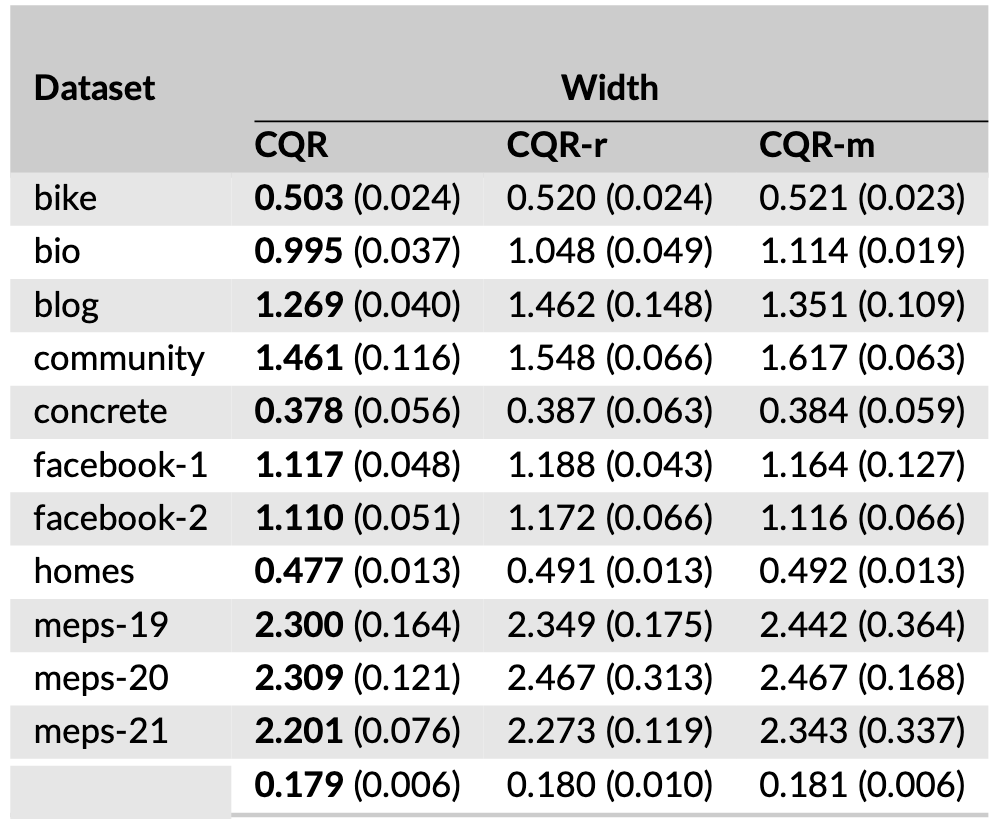
\includegraphics[width=\linewidth]{sesia_and_candes/tab_2.png}
            \caption{Table 2.}
            \label{fig:sesia_and_candes_tab_2}
        \end{subfigure}\hfill
        \begin{subfigure}{0.485\textwidth}
            \centering
            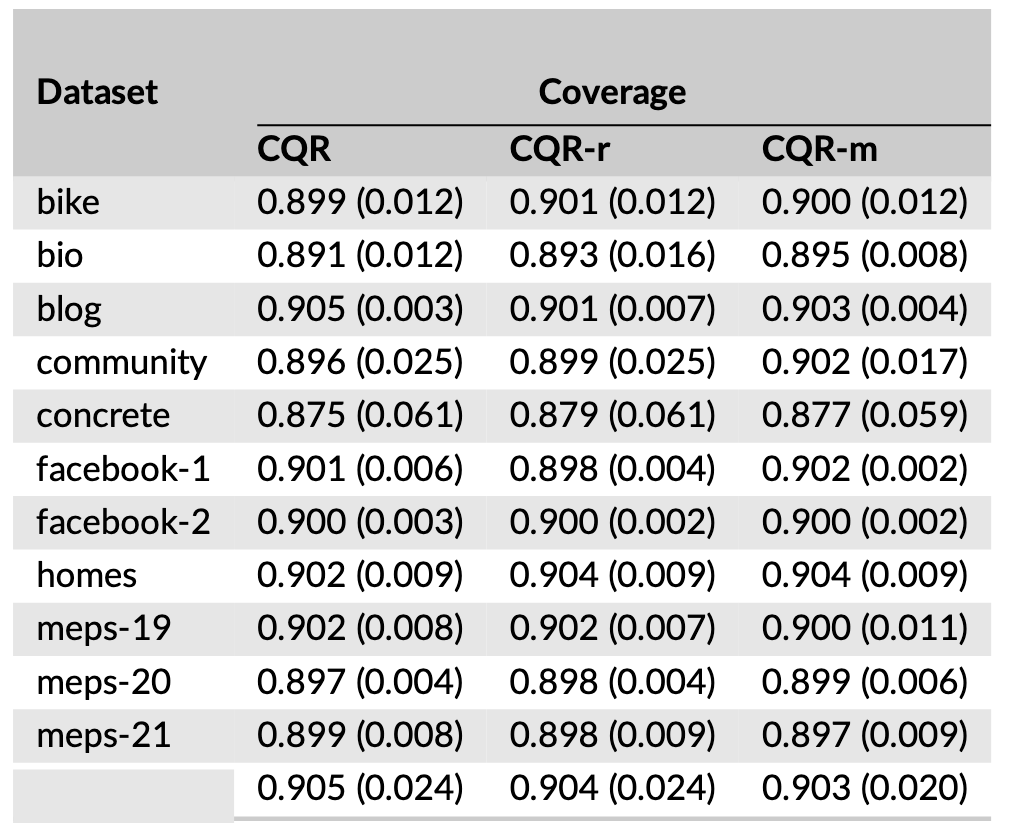
\includegraphics[width=\linewidth]{sesia_and_candes/tab_3.png}
            \caption{Table 3.}
            \label{fig:sesia_and_candes_tab_3}
        \end{subfigure}
        \caption{Tables 2 and 3 in \cite{sesia2020comp}}
        \label{fig:sesia_and_candes_tabs_2_3}
    \end{figure}

    \framebreak

    \begin{figure}
        \centering
        
\includegraphics[scale=0.23]{sesia_and_candes/fig_2.png}
        \caption{Figure 2 in \cite{sesia2020comp}.}
        \label{fig:sesia_and_candes_fig_2}
    \end{figure}
\end{frame}

\begin{frame}[allowframebreaks]{References}
    \bibliographystyle{agsm}
    \bibliography{bibliography}
\end{frame}

\end{document}